\documentclass[a4paper,11pt]{article}

%% We can use macros to avoid typing the same thing over and over
\newcommand{\token}[1]{\texttt{<#1>}}
\newcommand{\uC}{{$\mathrm{\mu}$}C }
 \usepackage{tikz}
 \usepackage{tikz-qtree}
 \usepackage{array}
\usepackage{amsmath}
\usepackage{multicol} 

\title{Assignment 2: Parser}
\author{Xiao Yang \and Magnus L{\aa}ng} % replace by your name(s)
\date{\today}
\begin{document}
\maketitle


\section{Technical Issues}
\subsection{Precedence of binary operators}
When rewrite the grammar to guarantee the precedence of operators, we first expand the production with low precedence operators and then the ones with high precedence.
For example, when considering \emph{plus} and \emph{multiply}, we use the following rules to enforce the precedence.
\begin{eqnarray*}
	& Expr \rightarrow Expr' + Expr' \\
	& Expr' \rightarrow Expr'' * Expr''
\end{eqnarray*}

\subsection{Associativity of binary operators}
\begin{itemize}
	\item \textbf{Left-Associative} \\
	For left-associative operators, we use the \emph{EBNF} form to rewrite the grammar.
	Also take expressions with \emph{plus} as an example, we write the following grammar rule:
	\begin{eqnarray*}
		Expr \rightarrow Expr' (+ Expr')*
	\end{eqnarray*}
	
	
	\item \textbf{Right-Associative} \\
	For right-associative operators, we adopt right recursive rules to build corresponding nodes.
	Take \emph{assignment} as an example, we write the following rule:
	\begin{eqnarray*}
		Expr \rightarrow Expr' = Expr
	\end{eqnarray*}
	
\end{itemize}


\newpage

\section{Appendix: AST Structure}
Here we present the nodes and their children of our Abstract Syntax Tree. Note that \emph{\#Expression} and \emph{\#Statement} are abstract node classes which are used to ease the representaion of the tree structure. The real nodes belong to these two classes are listed in the end.

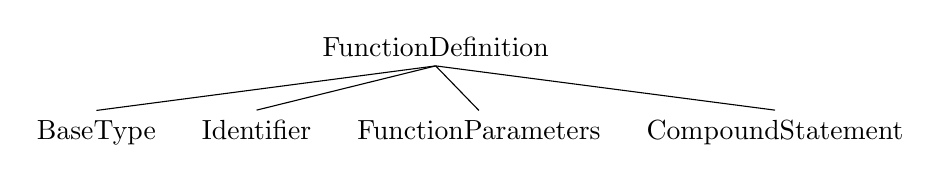
\begin{tikzpicture}[grow=down]
\tikzset{level distance = 30pt, sibling distance = 10pt}

\Tree [.FunctionDefinition
			[.BaseType ]
			[.Identifier ]
			[.FunctionParameters ]
			[.CompoundStatement ]
		]

\end{tikzpicture}

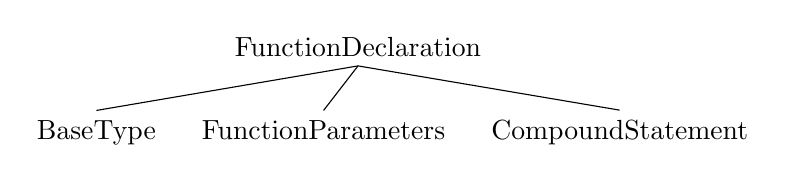
\begin{tikzpicture}[grow=down]
\tikzset{level distance = 30pt, sibling distance = 10pt}

\Tree [.FunctionDeclaration
			[.BaseType ]
			[.FunctionParameters ]
			[.CompoundStatement ]
		]

\end{tikzpicture}

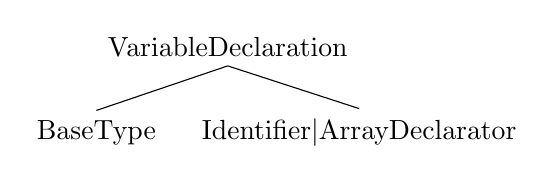
\begin{tikzpicture}[grow=down]
\tikzset{level distance = 30pt, sibling distance = 10pt}

\Tree [.VariableDeclaration
			[.BaseType ]
			[.Identifier$|$ArrayDeclarator ]
		]

\end{tikzpicture}


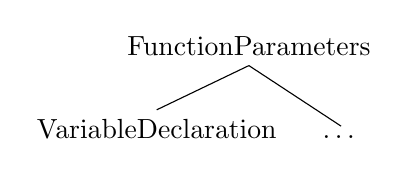
\begin{tikzpicture}[grow=down]
\tikzset{level distance = 30pt, sibling distance = 10pt}

\Tree [.FunctionParameters
			[.VariableDeclaration ]
			[.$\dots$ ]
		]

\end{tikzpicture}


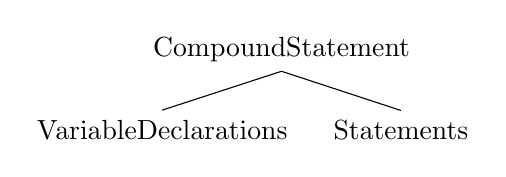
\begin{tikzpicture}[grow=down]
\tikzset{level distance = 30pt, sibling distance = 10pt}

\Tree [.CompoundStatement
			[.VariableDeclarations ]
			[.Statements ]
		]

\end{tikzpicture}

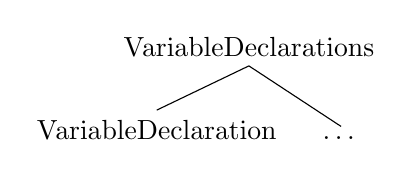
\begin{tikzpicture}[grow=down]
\tikzset{level distance = 30pt, sibling distance = 10pt}

\Tree [.VariableDeclarations
			[.VariableDeclaration ]
			[.$\dots$ ]
		]

\end{tikzpicture}

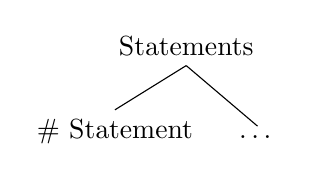
\begin{tikzpicture}[grow=down]
\tikzset{level distance = 30pt, sibling distance = 10pt}

\Tree [.Statements
			[.\#~Statement ]
			[.$\dots$ ]
		]

\end{tikzpicture}


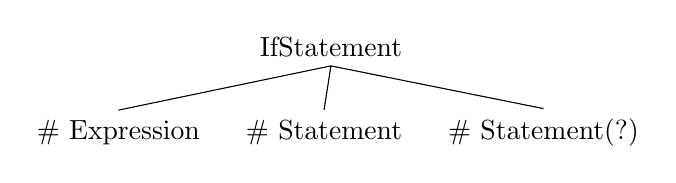
\begin{tikzpicture}[grow=down]
\tikzset{level distance = 30pt, sibling distance = 10pt}

\Tree [.IfStatement
			[.\#~Expression ]
			[.\#~Statement ]
			[.\#~Statement(?) ]
		]
\end{tikzpicture}

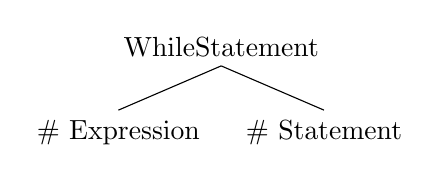
\begin{tikzpicture}[grow=down]
\tikzset{level distance = 30pt, sibling distance = 10pt}
\Tree [.WhileStatement
			[.\#~Expression ]
			[.\#~Statement ]
		]
\end{tikzpicture}

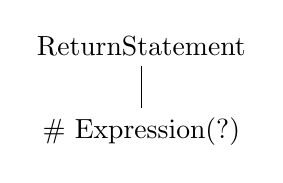
\begin{tikzpicture}[grow=down]
\tikzset{level distance = 30pt, sibling distance = 10pt}
\Tree [.ReturnStatement
			[.\#~Expression(?) ]
		]
\end{tikzpicture}


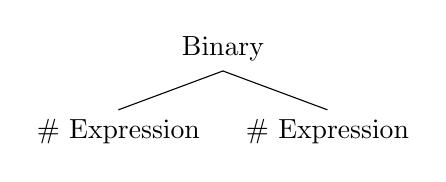
\begin{tikzpicture}[grow=down]
\tikzset{level distance = 30pt, sibling distance = 10pt}
\Tree [.Binary
			[.\#~Expression ]
			[.\#~Expression ]
		]
\end{tikzpicture}

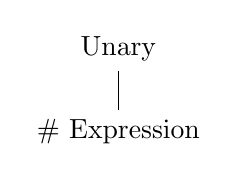
\begin{tikzpicture}[grow=down]
\tikzset{level distance = 30pt, sibling distance = 10pt}
\Tree [.Unary
			[.\#~Expression ]
		]
\end{tikzpicture}

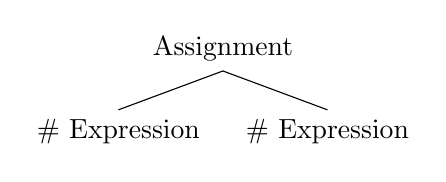
\begin{tikzpicture}[grow=down]
\tikzset{level distance = 30pt, sibling distance = 10pt}
\Tree [.Assignment
			[.\#~Expression ]
			[.\#~Expression ]
		]
\end{tikzpicture}

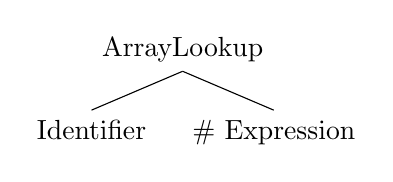
\begin{tikzpicture}[grow=down]
\tikzset{level distance = 30pt, sibling distance = 10pt}
\Tree [.ArrayLookup
			[.Identifier ]
			[.\#~Expression ]
		]
\end{tikzpicture}




\begin{multicols}{2}
\paragraph{\#~Statement} 
\begin{itemize}
	\item IfStatement 
	\item EmptyStatement 
	\item WhileStatement 
	\item CompoundStatement 
	\item ReturnStatement 
	\item \#~Expression 
\end{itemize}


\paragraph{\#~Expression} 
\begin{itemize}
	\item Binary 
	\item Assignment 
	\item Unary 
	\item IntegerLiteral 
	\item Identifier 
	\item ArrayLookup
\end{itemize}
\end{multicols}
	








\end{document}
